\chapter{Trabajo Relacionado}
\label{champ:relatedwork}
\bigskip
\barra
\bigskip

Existen varios algoritmos propuestos para la creación de redes porosas que siguen el MDSE y que solo están sujetos al $PC$. Entre 
los más sobresalientes están el m\'etodo BiaSED\cite{ref1} y el algoritmo NoMISS\cite{ref3}. En este cap\'itulo se presentar\'an
ambos algoritmos junto con sus respectivas versiones paralelas, descritas en \cite{ref4}, las cuales destacan 
debido a que permiten crear redes porosas de gran tamaño.\\

\section{Algoritmos Secuenciales}
\label{subsec:seqversions}
En esta sección se presentan dos algoritmos secuenciales para la creación de redes porosas sujetas \'unicamente al $PC$. El primer
algoritmo es de tipo iterativo, que hace uso del M\'etodo de Monte Carlo \cite{ref15} y el segundo algoritmo es un algoritmo voraz (o ávido)
que construye eficientemente redes porosas.\\

\subsection{Algoritmo BiaSED}
\label{subsubsec:biased}
El algoritmo BiaSED (Biased Simulation Early Design) se describe completamente en \cite{ref1} y \cite{ref4}. Se define como un 
algoritmo iterativo que se compone de tres pasos fundamentales. 

\begin{itemize}
\item[] \textbf{Paso 1}:
Se generan aleatoriamente los tamaños de los sitios 
($L^3$ tamaños de radios de sitios) y los enlaces ($3*L^3$ tamaños de radios de enlaces), en base a las 
distribuciones $F_S(R_S)$ and $F_B(R_B)$. Durante la generación, los valores 
son asignados al azar dentro del espacio c\'ubico de una red porosa.
La asignación se repite hasta que la red est\'e completamente inicializada. El resultado de este primer paso es una red porosa que 
probablemente no cumpla con el $PC$, especialmente cuando hay un alto traslape entre $F_S(R_S)$ y $F_B(R_B)$.\\
\item[] \textbf{Paso 2}:
Este consiste en la ejecución de una serie de Pasos de Monte Carlo ($MCs$) hasta que se genera una red válida. 
Un paso de Monte Carlo involucra $4L^3$ intercambios de tamaños de poros, lo anterior para lograr que las 
conexiones entre los poros sean válidas, es decir, que cumplan con el $PC$. Cada uno de los intercambios se hace cambiando el tamaño de 
dos sitios o dos enlaces, los cuales se seleccionan aleatoriamente; un intercambio es válido si y solo si el número de violaciones al 
$PC$ es menor o igual al número de violaciones existentes antes del intercambio, de lo contrario el intercambio es rechazado.\\
\item[] \textbf{Paso 3}:
Se aplica un n\'umero adicional de $MCs$ para mejorar la isotrop\'ia de la red porosa. El mejoramiento de la isotrop\'ia 
hace que las redes adquieran una distribuci'on de poros m\'as representativa de las redes porosas reales.  
\end{itemize}


\subsection{Algoritmo NoMISS}
\label{subsubsec:nomiss}
NoMISS (No Mistake Initial Seeding Situation) es un algoritmo voraz que trabaja con pequeñas soluciones válidas y que a través de 
iteraciones llega a una solución válida completa, este algoritmo se describe completamente en \cite{ref3}. El método se puede separar
en cuatro pasos fundamentales:

\begin{itemize}
\item[] \textbf{Paso 1. Generación de Poros}: se crean dos listas de sitios $L_{S}$ y $L_{SC}$. Los tamaños de radios de los sitios ($L^3$ radios)
son generados de forma aleatoria (en base a la distribución $F_S(R_S)$), los radios se ordenan de forma ascendente y se almacenan en la lista 
etiquetada como $L_{S}$. 
Después se generan los radios de los enlaces  de forma aleatoria (en base a la distribución $F_B(R_B)$). En adelante usaremos el t\'ermino 
sitio o enlace para referirnos al radio del sitio o del enlace, respectivamente. Por cada enlace generado, 
este se intenta conectar al primer sitio de la lista $L_{S}$ (al m\'as pequeño de la lista), mientras se cumpla el $PC$. Si no es posible, 
el enlace se intenta conectar con el siguiente sitio en $L_{S}$, y así sucesivamente hasta que la conexión cumpla el $PC$. Cada vez que 
un sitio en $L_{S}$ completa su contorno, es decir tiene $C=6$ enlaces conectados, el sitios es trasladado al final de la lista etiquetada 
como $L_{SC}$ la cual conserva el orden ascendente de los radios de sitios. Al final, $L_{SC}$ contiene sitios 
con sus respectivos seis enlaces válidos y $L_{S}$ contiene sitios con conexiones incompletas. Todos los enlaces conectados 
tanto en los sitios de $L_{SC}$ como en los de $L_{S}$ siempre cumplen el $PC$.\\

\item[] \textbf{Paso 2. Sembrado}: en este paso se eligen $k$ semillas (es decir $k$ sitios) tomadas de forma aleatoria de la lista $L_{SC}$, y 
son insertadas en posiciones aleatorias de la red, entonces los otros sitios de $L_{SC}$ son insertados alrededor de cada semilla, generando
así estructuras cúbicas (clusters c\'ubicos de poros) hasta logar el tamaño establecido como el cluster-size. En la Figura \ref{fig:cluster_nomiss}  se muestra la 
construcción de un cluster de tamaño 3x3x3. Cuando un sitio es conectado a otro sito en un cluster, solo se 
necesita de un enlace para su conexión (el cual debe de cumplir con el $PC$). Cuando dos enlaces se encuentran frente a frente para conectar 
dos sitios y los dos enlaces cumplen con el $PC$, el enlace de mayor tama\~no es elegido para la conexi\'on; de otra forma, se elige el enlace 
m\'as pequeño el cual permite que el $PC$ se cumpla en ambos extremos del enlace. El enlace sobrante es asignado a otro sitio en $L_{S}$, 
siguiendo el mismo procedimiento del Paso 1.\\

\item[] \textbf{Paso 3. Rellenado}: una vez terminado el proceso de siembra se comienza el rellenado de los espacios vacíos de la red, esto se realiza 
seleccionando aleatoriamente una de las semillas iniciales y se hace crecer su cluster hasta que se ocupen todos los espacios vacíos de la red.
Se hace notar que, si un espacio ya ha sido previamente inicializado, éste es descartado, considerando solamente los espacios vacíos.

\item[] \textbf{Paso 4. Mejoramiento de isotrop\'ia}: en este punto, igual que en el algoritmo BiaSED, la red porosa ya es v\'alida y solo hay que 
aplicar un n\'umero adicional de $MCs$ para mejorar su isotrop\'ia.
\end{itemize}

\begin{figure}[hbtp]
\centering
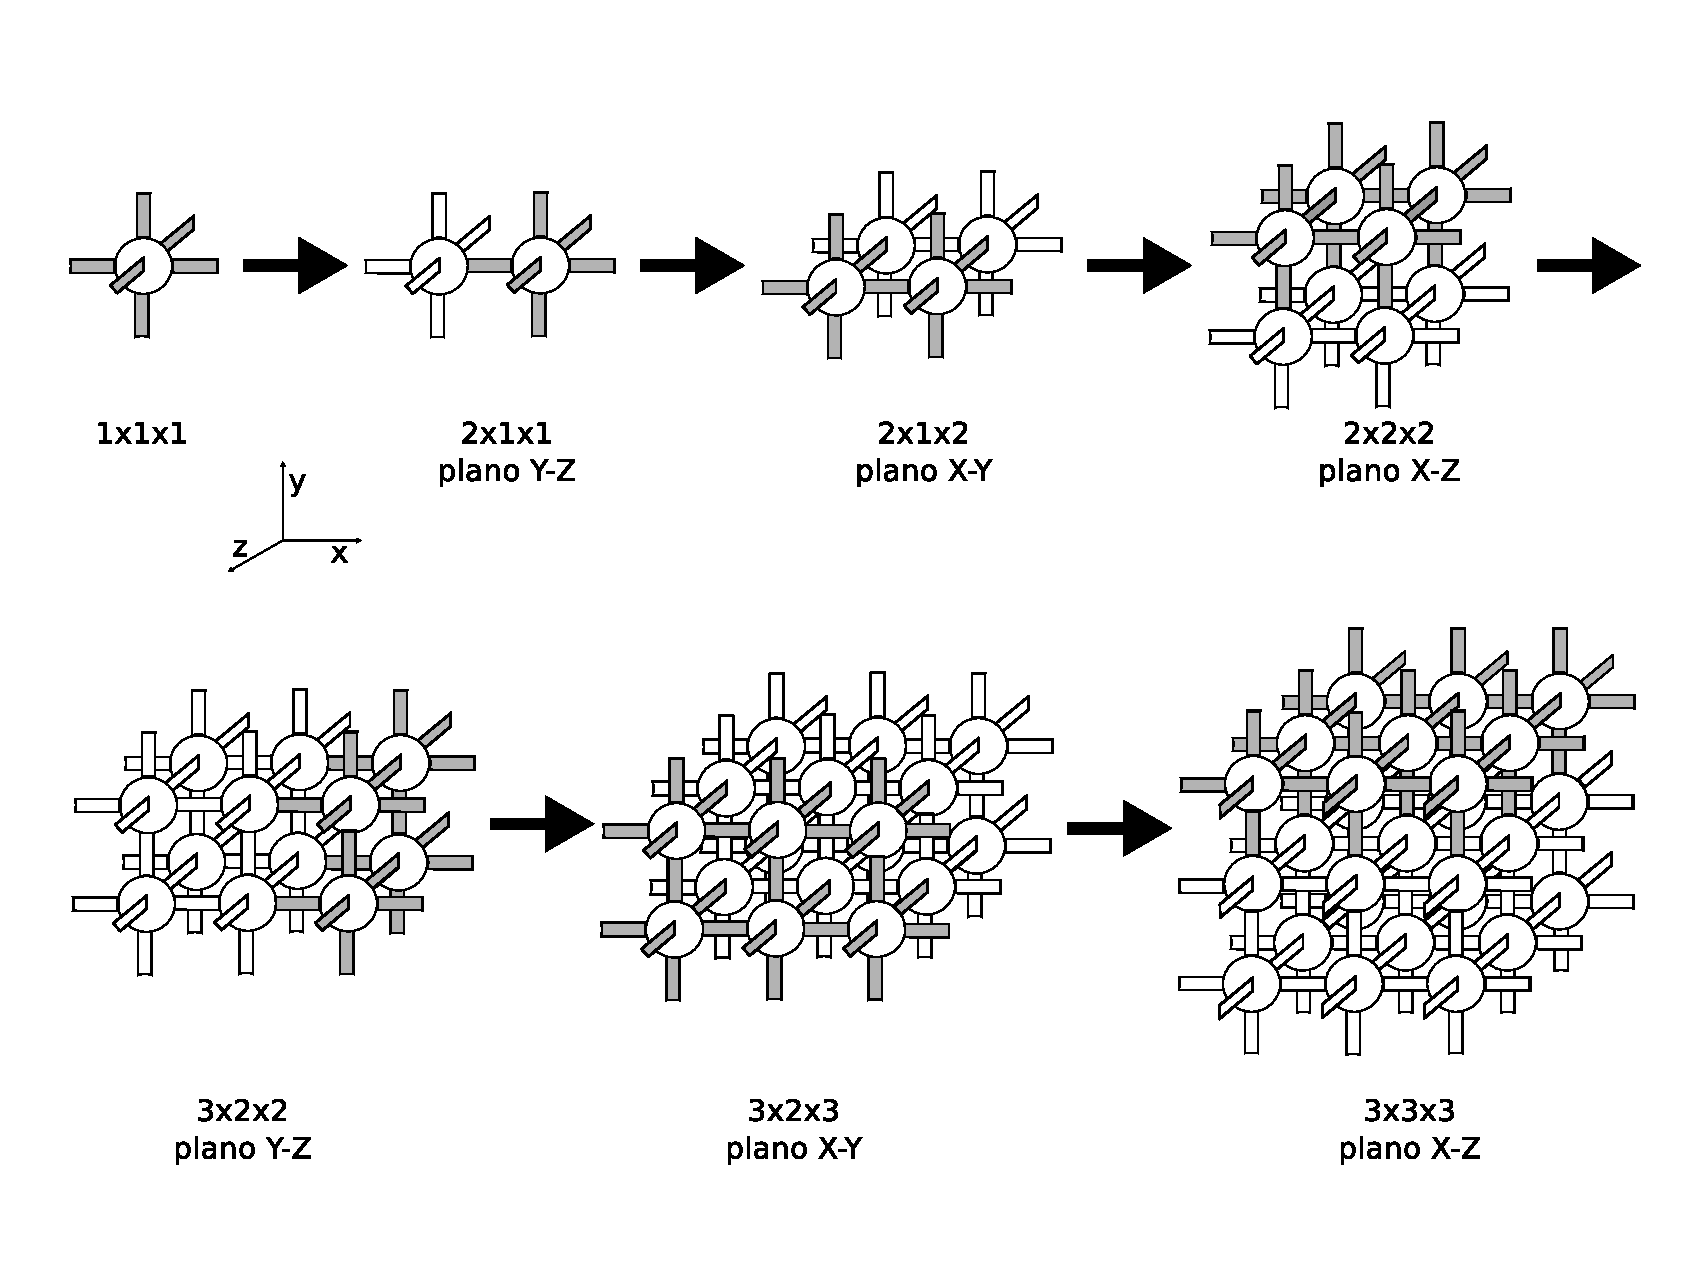
\includegraphics[width=5.0in]{img/cluster-nomiss_es.pdf}
\caption{Construcción de un cluster de tamaño 3x3x3 con el algoritmo NoMISS}
\label{fig:cluster_nomiss}
\end{figure}

El Algoritmo NoMISS a diferencia del BiaSED, no hace uso de los pasos de Monte Carlo, sino que crea desde el inicio una red porosa válida.\\
Estos algoritmos que se acaban de presentar ofrecieron buenos resultados al construir redes porosas que respetan el $PC$; sin 
embargo, ambos algoritmos necesitan tiempos largos para construir redes grandes. Debido a esto, hubo propuestas de paralelización de los
dos algoritmos; en esta sección se presenta una descripción breve de las versiones paralelas de BiaSED y NoMISS, las cuales se encuentran 
descritas a detalle en \cite{ref4}.


\section{Algoritmos Paralelos}
\label{subsec:algspar}

Las versiones paralelas de BiaSED y NoMISS están diseñadas para trabajar bajo el modelo de Paso de Mensajes, utilizando la tecnología de 
Message Passing Interface(MPI-C). En cada versión paralela la red es particionada en pequeñas subredes, como se observa en la 
Figura \ref{fig:distribucion_rw}; esta división se hace en base al número de nodos a utilizar, cada nodo tiene una subred 
de tamaño $L_x \cdot L_y \cdot L_z$, dicha distribución se hace utilizando funciones especificas de MPI. Los nodos mantienen 
una topología tipo toro, esto para crear una interconexión entre las distintas subredes. Para la explicación de los algoritmos se
 establece que un nodo es representado por un proceso MPI, por lo que utilizaremos indistintamente ambos términos.

\subsection{Algoritmo Paralelo BiaSED}
\label{subsubsec:pbiased}
El algoritmo BiaSED-paralelo se describe completamente en \cite{ref4}. Tal y como se coment\'o al inicio de esta secci\'on, la red 
porosa se divide en subredes las cuales se distribuyen entre los nodos de un cluster utilizando la tecnología de MPI, 
como vemos en la Figura \ref{fig:distribucion_rw} al utilizar 8 procesos. A continuación se describen a grandes rasgos los pasos del
funcionamiento de este algoritmo.

\begin{itemize}
\item[] \textbf{Paso 1}: Cada proceso genera $L^3/N$ sitios y $3L^3/N$ enlaces, donde $N$ es el número de procesos a utilizar. 
Cada proceso ejecuta el paso uno del algoritmo secuencial BiaSED trabajando en su respectivo espacio de subred.

\item[] \textbf{Paso 2}: Lo siguiente es que cada proceso ejecuta una serie de $MCs$ sobre su subred, a esto se le llama $MCs$ paralelo.
Este proceso se realiza excluyendo a los sitios ubicados en las caras exteriores de la subred, ya que dichos elementos no cuentan
con sus 6 enlaces y no podría validarse el $PC$.

\item[] \textbf{Paso 3}: Para que cada poro tenga la posibilidad de intercambiarse con otro de una subred distinta, se realiza una 
transferencia parcial de subred hacia una direcci\'on espec\'ifica ($x$, $y$ o $z$), entre los nodos del toro que tienen subredes vecinas. 
De esta manera, los sitios de las caras exteriores quedan ahora en la parte interna de una nueva subred. 

\item[] \textbf{Paso 4}: Los Pasos 2 y 3 son repetidos, alternando los ejes $x$, $y$ y $z$, hasta que se obtiene una red porosa válida.
\item[] \textbf{Paso 5}: En este última parte los Pasos 2 y 3 son repetidos por un n\'umero determinado de veces, para mejorar la isotrop\'ia
de la red porosa.
\end{itemize}

\begin{figure}[hbtp]
\centering
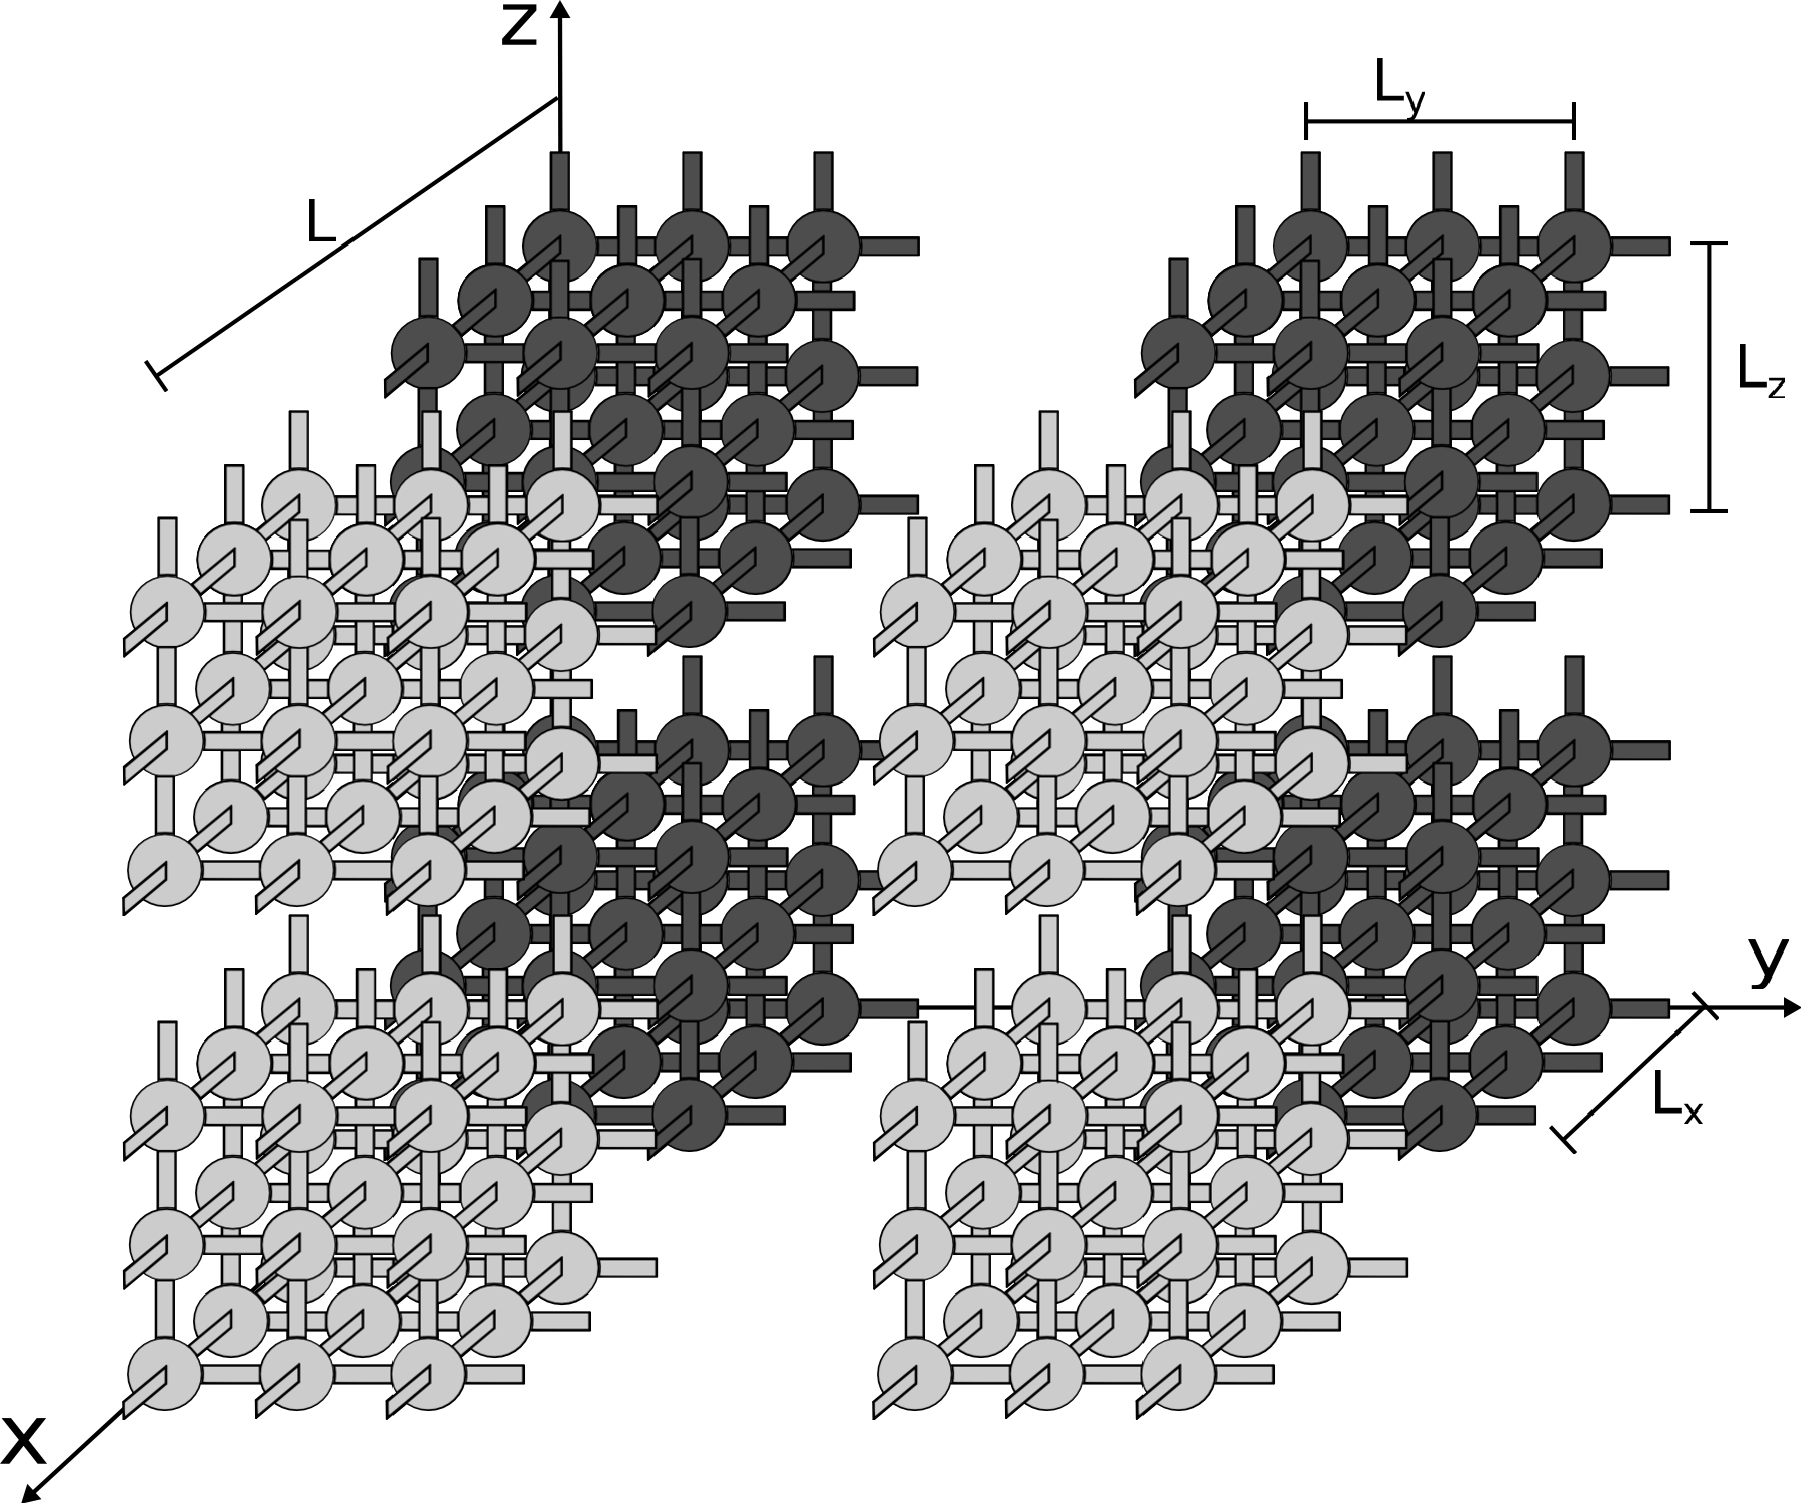
\includegraphics[width=2.8in]{img/distribucion}
\caption{Distribución de una red porosa entre 8 nodos o procesos MPI}
\label{fig:distribucion_rw}
\end{figure}

\subsection{Algoritmo Paralelo S-NoMISS}
\label{subsubsec:ps-nomiss}
El algoritmo paralelo S-NoMISS se describe con mayor detalle en \cite{ref3}, y est\'a basado en el algoritmo NoMISS descrito en la sección 
anterior. Este algoritmo paralelo se distingue por utilizar un método estático para la distribución de carga, 
lo pasos del algoritmo son los siguientes:

\begin{itemize}
\item[] \textbf{Paso 1. Generación de poros}: Cada nodo genera $L^3/N$ sitios y $3L^3/N$ enlaces, donde $N$ es el número de nodos a utilizar. Los 
sitios se ordenan de forma ascendente (aplicando el algoritmo Parallel-Quicksort). De este modo cada nodo crea las listas locales 
$L_S$ y $L_{SC}$, de la misma forma en que se hace en el Paso 1 del algoritmo NoMISS.

\item[] \textbf{Paso 2. Sembrado y Rellenado}: Cada nodo ejecuta sobre su subred el paso de sembrado y rellenado del algoritmo NoMISS secuencial,
con la restricción de que se omite la inicialización en posiciones ubicadas en las caras externas de cada subred.

\item[] \textbf{Paso 3. Rellenado de caras externas}: Para rellenar los espacios vacíos existentes entre las subredes y lograr cumplir 
el $PC$ entre las fronteras de las subredes adyacentes, se realizan un serie de trasferencias parciales de subred entre nodos, 
a lo largo de los ejes $x$, $y$ y $z$ del toro. Entre cada transferencia se aplica el método de rellenado, para que los espacios vac\'ios
que ahora quedaron en la parte interna de una subred 
se vayan inicializando, respetando el $PC$. Al terminar las transferencias, se tiene una red porosa válida, sin posiciones vac\'ias.

\item[] \textbf{Paso 4. Mejoramiento de isotrop\'ia}: En esta \'ultima parte se aplica el mismo Paso 5 del método BiaSED-paralelo, para mejorar 
la isotrop\'ia de la red porosa.
\end{itemize}

Debido a que en este algoritmo los sitios de mayor tamaño quedaban siempre en la parte exterior de la red porosa, era muy dif\'cil
mejorar la isotrop\'ia de la red, sobre todo cuando se tenían translapes $\Omega$ muy altos. Por tal motivo se propuso una nueva versi\'on
paralela de NoMISS, D-NoMISS, que permiti\'o que los sitios de mayor tama\~no pudieran distribuirse a lo largo de todo el espacio de la red, 
como lo hace la versi\'on secuencial NoMISS.  

\subsection{Algoritmo Paralelo D-NoMISS}
\label{subsubsec:pd-nomiss}
El algoritmo paralelo D-NoMISS se describe con mayor detalle en \cite{ref4}, este algoritmo ejecuta los pasos del algoritmo S-NoMISS 
con algunas modificaciones. Los pasos de D-NoMISS son los sigientes:

\begin{itemize}
\item[] \textbf{Paso 1. Generación de poros}: Aquí cada proceso ejecuta simuilt\'aneamente el mismo paso 1 de S-NoMISS.

\item[] \textbf{Paso 2. Sembrado paralelo}: En este paso, el sembrado paralelo de sitios se realiza casi igual que en S-NoMISS, en donde
cada proceso omite las caras externas de su subred; lo que cambia ahora es el espacio en donde las semillas son asignadas y agrandadas en
clusters c\'ubicos de poros. Para que cada poro tenga la
posibilidad de ser sembrado en cualquier parte de la red porosa, los procesos trasfieren la mitad de su subred a sus respectivos vecinos 
en el toro (en las tres direcciones $x$, $y$ y $z$), y entre cada trasferencia se realiza una siembra paralela de sitios. De esta manera 
los espacios en las caras externas tambi\'en podr\'ian ser inicializados durante el sembrado.
Los clusters de poros ocupan hasta el $25\%$ de la subred. Cabe destacar que las listas $L_{SC}$ locales de cada nodo, al terminar el
sembrado paralelo no son necesariamente del mismo tamaño, debido a los translapes de clusters que posiblemente ocurrieron durante el proceso.

\item[] \textbf{Paso 3. Rellenado paralelo}: Cada proceso intenta llenar los lugares vacíos de su subred mediante un cluster recubridor que 
inicia desde el centro de la subred y que se 
extiende hasta un tamaño $(L_x -2) \cdot (L_y - 2) \cdot (L_z -2)$, excluyendo las caras externas de la subred. Debido al paso dos y 
las posibilidad de que las listas $L_{SC}$ sean de distintos tamaños, cada vez que un proceso se queda sin sitios que asignar, se 
ejecuta una política de distribución de carga que hace que las listas de poros permanezcan equilibradas, respecto al n\'umero de sitios que 
contienen. Igual que en el paso 3 de S-NoMISS, para inicializar todos los espacios vac\'ios se realizan un serie de trasferencias parciales de 
subred entre nodos, a lo largo de los ejes $x$, $y$ y $z$ del toro, y entre cada transferencia se construye un cluster recubridor.

\item[] \textbf{Paso 4. Mejoramiento de isotrop\'ia}: Como en todos los algoritmos descritos anteriormente, se recomienda aplicar un 
número adicional de $MCs$ para mejorar la isotropía de la red porosa; esto se hace de la misma forma que el Paso 4 de S-NoMISS.\\
\end{itemize}

%\section{Computo paralelo sobre memoria compartida}
%\label{sec:rwconclutions}

\section{Conclusiones}
\label{sec:rwconclutions}
En general se ha mostrado que los algoritmos NoMISS tienen mejor rendimiento que los algoritmos BiaSED \cite{ref3}, especialmente cuando se pretende construir redes porosas con alto traslape ($\Omega$). En cuanto a las versiones paralelas de NoMISS la versión S-NoMISS se observa mejor  en términos de tiempo; sin embargo en términos de la ísotropía de la red el algoritmo D-NoMISS es mejor, el mayor problema de la versión  D-NoMISS es que su método de distribución dinámica genera un punto de sincronizaci\'on global que hace que su escalabilidad sea limitada.\\

El inconveniente de estas versiones es que \'unicamente toman en cuenta el cumplimiento del Principio de Construcci\'on, por lo que  es de gran inter\'es el desarrollo de simuladores de redes porosas que consideren tambi\'en el cumplimiento de las  Retricciones Geom\'etricas ($RG$) durante la interconexión de poros. En \cite{ref5} se muestra una primera aproximación para 
la creación de redes porosas las cuales cumplen  completamente con el $PC$ y las $RG$; sin embargo, el método propuesto result\'o ser una solución impráctica ya que requería de grandes tiempos de ejecución para la generación de redes porosas de tamaños de red relativamente pequeños(que contenían a lo más $40^3$ poros).\\

En b\'usqueda de algoritmos eficientes que consideren el cumplimiento de ambas restricciones, $PC$ y $RG$, se implement\'o y se evaluó una adaptaci\'on del algoritmo secuencial NoMISS \cite{ref16} para crear redes de poros que cumplan con los dos tipos de retricciones. Sin embargo, debido a que los enlaces y sitios se generan de forma aleatoria 
fue muy difícil encontrar configuraciones válidas, lo que se trasformaba en tiempos de ejecución muy altos y como resultado solo 
se logro generar redes porosas con traslapes muy pequeños ($\Omega<=0.0007$) utilizando este esquema. En base al resultado 
anterior no se intent\'o paralelizar dicha versión ya que la limitante del traslape afectaría de igual forma a una versión paralela.\\

Para resolver este problema, inspirados por el funcionamiento de NoMISS y BiaSED, se propuso una nueva  solución \cite{ref17} para la construcción de redes prosas más reales considerando las Restricciones Geométricas. En \cite{ref17} se propone un algoritmo secuencial h\'ibrido que inicialmente ejecuta un procedimiento 
tipo voraz para inicializar la red y posteriormente aplica un m\'etodo iterativo para eliminar las violaciones a las restricciones de $PC$ y $RG$.
La desventaja de este algoritmo son sus tiempos de ejecuci\'on para crear redes de gran tama\~no debido a procesos de ordenamiento y
de b\'usqueda que tuvieron que incluirse.\\

En este trabajo se proponen dos versiones paralelas para la construcci\'on de redes porosas que consideran el cumplimiento de $PC$ y $RG$.
La primer versi\'on se refiere a la paralelizaci\'on del algoritmo h\'ibrido presentado en \cite{ref17}. Para tener otro punto 
de comparaci\'on tambi\'en se propuso una adaptaci\'on al algoritmo BiaSED-paralelo para que considerara los dos tipos de restricciones.
Ambas propuestas fueron desarrolladas utilizando las arquitecturas multi-núcleo, para sacar el mayor provecho de la memoria compartida
entre procesadores. Como trabajo futuro ser\'ia de gran inter\'es desarrollar estas versiones considerando arquitecturas de memoria distribuida
y as\'i ampliar el panorama comparativo. Las versiones paralelas de NoMISS y BiaSED se toman únicamente como antecedentes y no como un punto de partida o comparación, ya que el trabajo propuesto se refiere a un algoritmo diferente el cual toma en cuenta el cumplimiento de las $RG$. \\

En los Capítulos \ref{champ:BSGR} y \ref{champ:PBSGR} se presentar\'an respectivamente el algoritmo secuencial h\'ibrido propuesto en \cite{ref17} y los algoritmos paralelos propuestos en este trabajo.


